\Section{Непрерывность функции в точке. Свойства функций, непрерывных в точке.
Односторонняя непрерывность. Непрерывность сложной функции.
Теорема о переходе к пределу под знаком непрерывной функции.
Точки разрыва, их классификация. Разрывы монотонных функций}

\Subsection{Непрерывность функции в точке. Свойства функций, непрерывных в точке.
Односторонняя непрерывность}

\begin{definition}
Функция \(f(x)\) называется \textit{непрерывной в точке \(x_{0}\)}, если предел функции
в этой точке существует и равен \(f(x_{0})\).
\[
[ f(x) - \text{ непрерывная в } x_{0} ] \overset{def}{=}
\Big[ \lim_{ x \to x_{0} } f(x) = f(x_{0}) \Big]
\]
\end{definition}

\begin{definition}
Функция \(f(x)\) называется \textit{непрерывной справа (слева) в точке \(x_{0}\)},
если предел справа (слева) функции в этой точке существует и равен \(f(x_{0})\).
\[
[ f(x) - \text{ непрерывная справа (слева) в } x_{0} ] \overset{def}{=}
\Big[ f(x_{0} \pm 0) = f(x_{0}) \Big]
\]
\end{definition}

\begin{statement}
Если функция \(f(x)\) непрерывна слева и справа в точке \(x_{0}\),
то она непрерывна в этой точке.

\medskip

\proofname~По определению непрерывности слева и справа \(f(x_{0} - 0) = f(x_{0} + 0)\).
\text{По Утверждению \ref{statement_side_lims}} получаем, что и (неодносторонний) предел
функции \(f(x)\) существует в точке \(x_{0}\), причем выполняется
\[
\lim_{ x \to x_{0} } f(x) = \lim_{ x \to x_{0} \pm 0} f(x) = f(x_{0}).
\]
Следовательно, по определению функция \(f(x)\) непрерывна в \(x_{0}\).~\qedsymbol
\end{statement}

\begin{theorem}
Пусть функции \(f(x)\) и \(g(x)\) заданы в некоторой \(\Delta\)-окрестности точки \(x_{0}\)
и непрерывны в этой точке. Тогда функции \(y = f(x) \pm g(x), ~ y = f(x) \cdot g(x)\)
и \(y = \dfrac{f(x)}{g(x)}\) непрерывны в точке \(x_{0}\) (в случае частного \(g(x_{0}) \neq 0\)).

\medskip

\proofname~Докажем для суммы (разности),
поскольку для остальных операций доказательства аналогичны. \\
Изначально по условию непрерывности имеем:
\[
\lim_{ x \to x_{0} } f(x) = f(x_{0}) \qquad \& \qquad \lim_{ x \to x_{0} } g(x) = g(x_{0}).
\]
По Теореме \ref{theorem_lim_arithmetic} предел суммы (разности) функций существует
и равен сумме (разности) пределов. Следовательно, получаем:
\[
\lim_{ x \to x_{0} } (f(x) + g(x)) = \lim_{ x \to x_{0} } f(x) + \lim_{ x \to x_{0} } g(x) =
f(x_{0}) + g(x_{0})
\]
Следовательно, по определению непрерывности функция \(y = f(x) + g(x)\)
также непрерывна в точке \(x_{0}\).~\qedsymbol
\end{theorem}

\Subsection{Теорема о переходе к пределу под знаком непрерывной функции.
Непрерывность сложной функции}

\begin{theorem}[Теорема о переходе к пределу под знаком непрерывной функции]
\label{theorem_continuity_composition}
Пусть функция \(f(x)\) определена в некоторой проколотой окрестности точки \(x_{0}\)
и существует предел \(\lim\limits_{x \to x_{0}} f(x) = \alpha\).
Функция \(g(y)\) определена в некоторой окрестности точки \(\alpha\)
и непрерывна в этой точке. Тогда выполняется равенство:
\[
\lim_{ x \to x_{0} } g(f(x)) = g(\alpha).
\]

\medskip

\proofname~Пусть \(\{x_{n}\}\)~--- произвольная последовательность Гейне, сходящаяся к \(x_{0}\).
Тогда последовательность \(\{f(x_{n})\}\) сходится к \(\alpha\). \\
По определению непрерывности получаем, что \(\lim\limits_{n \to \infty} g(f(x_{n})) = g(\alpha)\).
Поскольку мы брали произвольную последовательность Гейне,
то (согласно определению по Гейне) окончательно получаем
\[
\lim_{ x \to x_{0} } g(f(x)) = g(\alpha),
\]
что и требовалось доказать.~\qedsymbol
\end{theorem}

\begin{theorem}
Пусть функция \(f(x)\) непрерывна в точке \(x_{0}\), а функция \(g(y)\)
непрерывна в точке \(\alpha\), причем \(f(x_{0}) = \alpha\).
Тогда функция \(h(x) = g(f(x))\) непрерывна в точке \(x_{0}\).

\medskip

\proofname~По Теореме \ref{theorem_continuity_composition} имеем:
\[
\lim_{ x \to x_{0} } h(x) = \lim_{ x \to x_{0} } g(f(x)) = g(f(x_{0})) = h(x_{0}),
\]
\[
\lim_{ x \to x_{0} } h(x) = h(x_{0}),
\]
что и требовалось доказать.~\qedsymbol
\end{theorem}

\Subsection{Точки разрыва, их классификация}

\begin{definition}
Точка \(x_{0}\) называется \textit{точкой устранимого разрыва} функции \(f(x)\),
если существует конечный предел функции в точке \(x_{0}\), но функция либо не определена
в этой точке, либо \(\lim\limits_{x \to x_{0}} f(x) \neq f(x_{0})\).
\[
\Big[ \exists \, \lim_{ x \to x_{0} } f(x) \neq f(x_{0}) \Big] ~ \vee ~
\Big[ \exists \, \lim_{ x \to x_{0} } f(x), ~~ \nexists \, f(x_{0}) \Big].
\]
\end{definition}

\begin{definition}
Точка \(x_{0}\) называется \textit{точкой разрыва первого рода} функции \(f(x)\),
если существуют конечные левый и правый пределы функции в точке \(x_{0}\),
но эти пределы не равны.
\[
f(x_{0} - 0) \neq f(x_{0} + 0).
\]
\end{definition}

\begin{definition}
Точка \(x_{0}\) называется \textit{точкой разрыва второго рода} функции \(f(x)\),
если в этой точке не существует хотя бы одного \textit{конечного} одностороннего предела функции.
\[
\nexists \, f(x_{0} - 0) \qquad \vee \qquad \nexists \, f(x_{0} + 0).
\]
\end{definition}

\begin{center}
\begin{minipage}{0.32\textwidth}
\centering
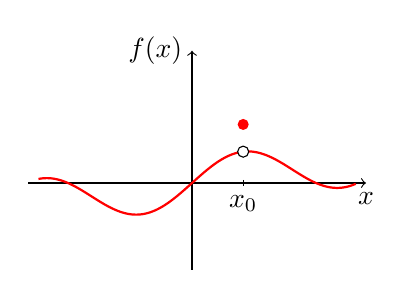
\begin{tikzpicture}[x=0.65cm,y=0.48cm]
\draw[->] (-3.2,0) -- (3.4,0) node[below] {$x$};
\draw[->] (0,-2.3) -- (0,3.5) node[left] {$f(x)$};

\draw[thick, smooth, red, domain=-3:1, samples=100]
plot (\x,{0.18*\x+0.65*sin(deg(1.6*\x))});
\draw[thick, smooth, red, domain=1:3.2, samples=100]
plot (\x,{0.18*\x+0.65*sin(deg(1.6*\x))});

\filldraw[fill=white]
(1,{0.18+0.65*sin(deg(1.6))}) circle (2pt);
\fill [red] (1,1.55) circle (2pt);

\draw (1,0.08) -- (1,-0.08);
\node[below] at (1,-0.08) {$x_0$};
\end{tikzpicture}
\textbf{Устранимый разрыв}
\end{minipage}
\hfill
\begin{minipage}{0.32\textwidth}
\centering
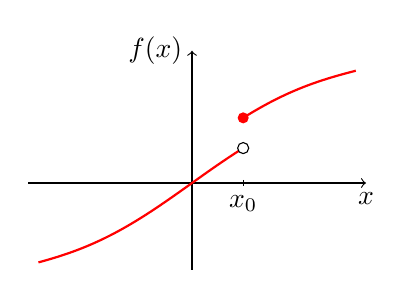
\begin{tikzpicture}[x=0.65cm,y=0.48cm]
\draw[->] (-3.2,0) -- (3.4,0) node[below] {$x$};
\draw[->] (0,-2.3) -- (0,3.5) node[left] {$f(x)$};

\draw[thick, smooth, red, domain=-3:1, samples=100]
plot (\x,{0.65*\x+0.35*sin(deg(0.9*\x))});
\draw[thick, smooth, red, domain=1:3.2, samples=100]
plot (\x,{0.65*\x+0.35*sin(deg(0.9*\x))+0.8});

\filldraw[fill=white]
(1,{0.65+0.35*sin(deg(0.9))}) circle (2pt);
\fill [red] (1,{1.45+0.35*sin(deg(0.9))}) circle (2pt);

\draw (1,0.08) -- (1,-0.08);
\node[below] at (1,-0.08) {$x_0$};
\end{tikzpicture}
\textbf{Разрыв первого рода}
\end{minipage}
\hfill
\begin{minipage}{0.32\textwidth}
\centering
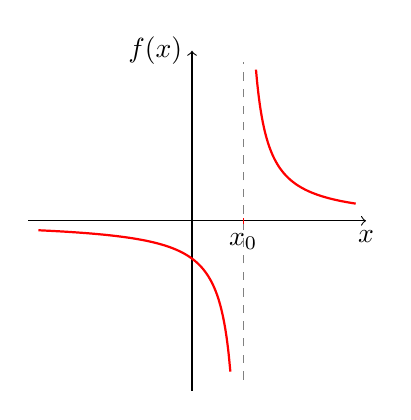
\begin{tikzpicture}[x=0.65cm,y=0.48cm]
\draw[->] (-3.2,0) -- (3.4,0) node[below] {$x$};
\draw[->] (0,-4.5) -- (0,4.5) node[left] {$f(x)$};

\draw[thick, smooth, red, domain=-3:0.75, samples=100]
plot (\x,{1/(\x-1)});
\draw[thick, smooth, red, domain=1.25:3.2, samples=100]
plot (\x,{1/(\x-1)});

\draw[dashed, gray] (1,-4.2) -- (1,4.2);
\draw [red] (1,0.08) -- (1,-0.08);
\node[below] at (1,-0.08) {$x_0$};
\end{tikzpicture}
\textbf{Разрыв второго рода}
\end{minipage}
\end{center}


\Subsection{Разрывы монотонных функций}

\begin{definition}
Функция \(f(x)\) называется \textit{непрерывной на интервале \((a, \, b)\)},
если она непрерывна в каждой точке этого интервала.
\end{definition}

\begin{theorem}
Если функция \(f(x)\) определена и монотонна на интервале \((a, \, b)\),
то она может иметь на этом интервале только точки разрыва первого рода.

\medskip

\proofname~По Теореме \ref{theorem_sideLims_monotonous} левый и правый пределы
функции в точке существуют~--- следовательно, разрывы второго рода исключены. \\
Предположим, что в точке \(x_{0}\) функция \(f(x)\) претерпевает устранимый разрыв.
Тогда левый и правый пределы равны:
\[
f(x_{0} - 0) = f(x_{0} + 0).
\]
Но по Теореме \ref{theorem_sideLims_monotonous} имеем:
\[
f(x_{0} - 0) \leq f(x_{0}) \leq f(x_{0} + 0).
\]
Отсюда получаем, что
\[
f(x_{0} - 0) = f(x_{0}) = f(x_{0} + 0).
\]
Но тогда в точке \(x_{0}\) вовсе нет разрыва~--- противоречие.
Следовательно, устранимые разрывы также исключены,
и возможными остаются только разрывы первого рода.~\qedsymbol
\end{theorem}

\begin{theorem}
Если функция \(f(x)\) определена и монотонна на интервале \((a, \, b)\),
то множество ее точек разрыва не более чем счетно.

\medskip

\proofname~Пусть функция \(f(x)\) неубывающая на интервале \((a, \, b)\).
Обозначим множество \(X\) как множество точек ее разрыва. \\
Согласно Теореме \ref{theorem_sideLims_monotonous} имеем:
\[
f(x_{0} - 0) \leq f(x_{0} + 0).
\]
Причем равенства быть не может, ведь иначе (см. доказательство предыдущей теоремы)
точка \(x_{0}\) вовсе не будет точкой разрыва. Тогда справедливо строгое неравенство
\[
f(x_{0} - 0) < f(x_{0} + 0).
\]
Тогда, поскольку \(f(x)\) неубывающая, весь интервал значений \((f(x_{0} - 0), \, f(x_{0} + 0))\)
за исключением, быть может, точки \(f(x_{0})\), не принадлежит множеству значений функции \(f(x)\).
Поскольку функция монотонна, то для произвольных неравных точек \(x_{1}\) и \(x_{2}\)
из множества \(X\) выполняется следующее:
\[
(f(x_{1} - 0), \, f(x_{1} + 0)) ~ \cap ~ (f(x_{2} - 0), \, f(x_{2} + 0)) = \emptyset.
\]
Иначе говоря, интервалы <<вырезанных>> значений не пересекаются.
Тогда по Лемме \ref{lemma_rational_in_real} найдется такое \textit{рациональное}
число \(c_{0}\), что \(f(x_{0} - 0) < c_{0} < f(x_{0} + 0)\). \\
Таким образом, мы взаимно однозначно сопоставили каждой точке разрыва свое рациональное число.
Следовательно, поскольку \(\Q\) счетно, а мы определили подмножество \(\Q\),
то множество \(X\) должно быть не более чем счетно.\\
Для невозрастающей функции доказательство аналогично.~\qedsymbol
\end{theorem}

\begin{center}
\begin{minipage}{0.49\textwidth}
\centering
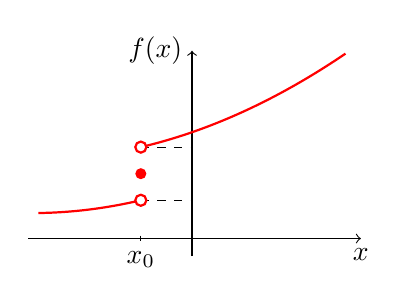
\begin{tikzpicture}[x=0.65cm,y=0.45cm]
\draw[->,black] (-3.2,0) -- (3.3,0) node[below] {$x$};
\draw[->,black] (0,-0.5) -- (0,5.3) node[left] {$f(x)$};

% Пунктир от границ разрыва до вертикальной оси
\draw[dashed,black] (-1,1.08) -- (0,1.08);
\draw[dashed,black] (-1,2.58) -- (0,2.58);

% Возрастающие ветви графика
\draw[thick,red,domain=-3:-1,samples=100]
plot (\x,{0.08*\x*\x+0.5*\x+1.5});
\draw[thick,red,domain=-1:3,samples=100]
plot (\x,{0.08*\x*\x+0.5*\x+3.0});

% Односторонние пределы и значение функции
\draw[thick,red,fill=white] (-1,1.08) circle (2pt);
\draw[thick,red,fill=white] (-1,2.58) circle (2pt);
\fill[red] (-1,1.83) circle (2pt);

\draw[black] (-1,0.08) -- (-1,-0.08);
\node[below] at (-1,-0.08) {$x_0$};
\end{tikzpicture} \\
\textbf{<<Вырезанный>> интервал с точкой \(f(x_{0})\)}
\end{minipage}
\hfill
\begin{minipage}{0.49\textwidth}
\centering
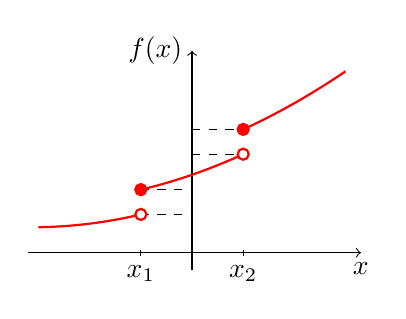
\begin{tikzpicture}[x=0.65cm,y=0.45cm]
\draw[->,black] (-3.2,0) -- (3.3,0) node[below] {$x$};
\draw[->,black] (0,-0.5) -- (0,5.7) node[left] {$f(x)$};

% Пунктир от границ разрывов до вертикальной оси
\draw[dashed,black] (-1,1.08) -- (0,1.08);
\draw[dashed,black] (-1,1.78) -- (0,1.78);
\draw[dashed,black] (0,2.78) -- (1,2.78);
\draw[dashed,black] (0,3.48) -- (1,3.48);

% Возрастающие ветви графика
\draw[thick,red,domain=-3:-1,samples=100]
plot (\x,{0.08*\x*\x+0.5*\x+1.5});
\draw[thick,red,domain=-1:1,samples=100]
plot (\x,{0.08*\x*\x+0.5*\x+2.2});
\draw[thick,red,domain=1:3,samples=100]
plot (\x,{0.08*\x*\x+0.5*\x+2.9});

% Односторонние пределы в точках разрыва
\draw[thick,red,fill=white] (-1,1.08) circle (2pt);
\draw[thick,red,fill=red] (-1,1.78) circle (2pt);
\draw[thick,red,fill=white] (1,2.78) circle (2pt);
\draw[thick,red,fill=red] (1,3.48) circle (2pt);

\draw[black] (-1,0.08) -- (-1,-0.08);
\draw[black] (1,0.08) -- (1,-0.08);
\node[below] at (-1,-0.08) {$x_1$};
\node[below] at (1,-0.08) {$x_2$};
\end{tikzpicture} \\
\textbf{<<Вырезанные>> интервалы не пересекаются}
\end{minipage}
\end{center}